\subsection{Ray tracing simulations}

\textbf{You will:}

\begin{itemize}
    \item Simulate wigglers 
\end{itemize}

\textbf{Questions:}

\textbf{i)} Simulate the wiggler for the ESRF ID19 in the energy interval 10000$\pm$10~eV. Estimate the total horizontal divergence looking at the velocity plot and compare with the  width of the $x'$ histogram. Visualize a top view of the emission (y,x) with and without emittance. Input data is in table~\ref{tab:electron_params}.

\begin{table}[h]
\centering
\caption{Electron and wiggler Parameters for ID19.}
\begin{tabular}{lcc}
\hline
\textbf{Parameter} & \textbf{Value} & \textbf{Unit} \\
\hline
$\sigma_x$ & 31.16 & $\mu$m \\
$\sigma_y$ & 5.16 & $\mu$m \\
$\sigma_{x'}$ & 4.52 & $\mu$rad \\
$\sigma_{y'}$ & 1.94 & $\mu$rad \\
Electron beam energy & 6.0 & GeV \\
Electron current & 0.200 & A \\
\hline
Period length & 0.15 & m \\
Number of periods & 6.867 & --- \\
Horizontal $K$ & 0.0 & --- \\
Vertical $K$ & 20.4911 & --- \\
\hline
\end{tabular}
\label{tab:electron_params}
\end{table}

 

\textbf{Hints:} you may use the workspace file {\tt wigglers.ows}

\textbf{Answer}

\begin{figure}[H]
\label{fig:id-fig1}
\caption{Electron transversal velocity (left) trajectory (right). Note that the velocities are centred, but not the trajectories. By default, the electron enters the wiggler at $x=0$.}

\includegraphics[width=0.49\textwidth]{wigglers/fig1a.png}

\includegraphics[width=0.49\textwidth]{wigglers/fig2a.png}
\end{figure}


\begin{figure}[H]
\label{fig:id-fig2}
\caption{Electron trajectory (left), and source emission. Note that the non-centered trajectory imply that the photon source is not centered at zero. This is ``corected" in next figure.}

\includegraphics[width=0.49\textwidth]{wigglers/fig2a.png}

\includegraphics[width=0.49\textwidth]
{wigglers/fig2b.png}
\end{figure}


\begin{figure}[H]
\label{fig:id-fig2bis}
\caption{Electron trajectory corrected to place the center at ``half-excursion" (left), and source emission. Note that the centered trajectory imply that the photon source is now centered at zero.}
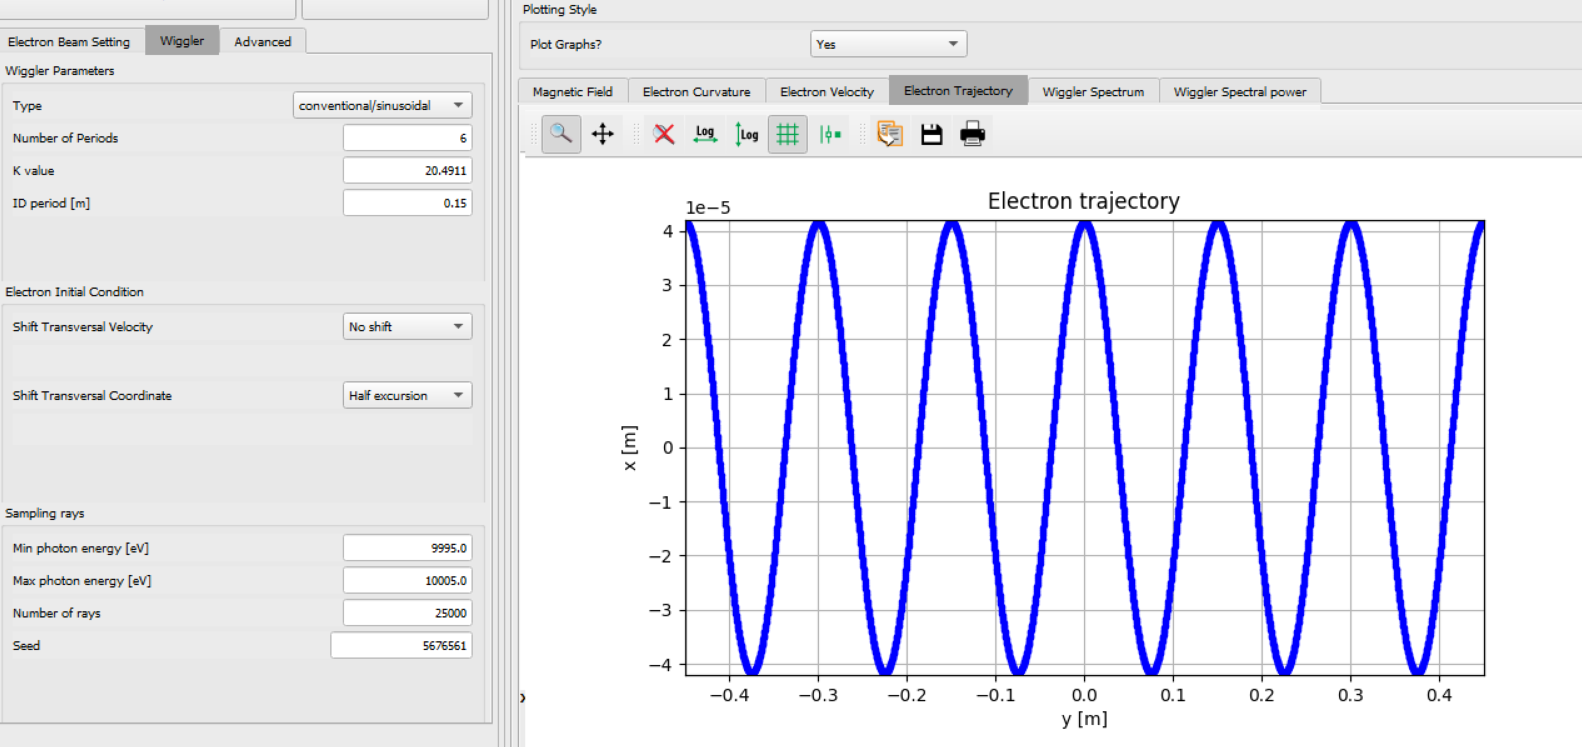
\includegraphics[width=0.49\textwidth]{wigglers/fig2c.png}
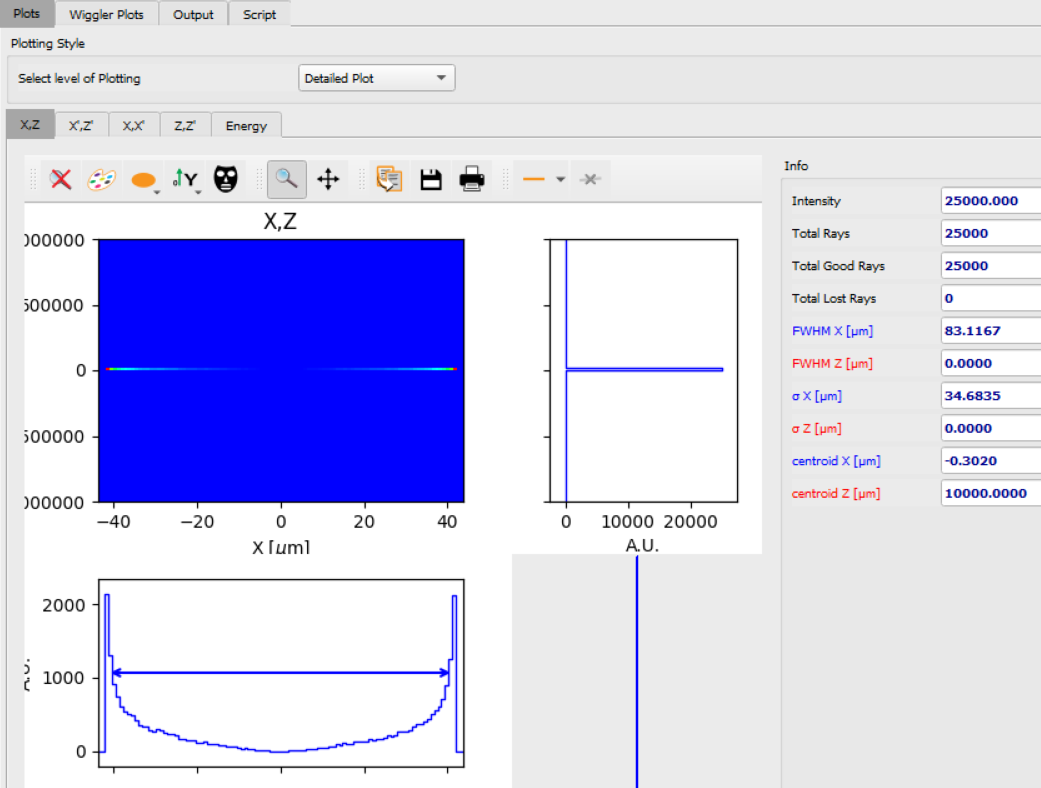
\includegraphics[width=0.49\textwidth]
{wigglers/fig2d.png}
\end{figure}

\begin{figure}[H]
\label{fig:id-fig3}
\caption{Phase space (X,X') at the source. Left: The default play displays the (X', Z') coordenates, therefore ignoring the effect Y coordinate (depth). Right: by doing "retrace" the rays are propagated to the plane $y=0$, thus considering the depth of the source. This produces the typical ``star" phase-space in the wigglers.}

\includegraphics[width=0.49\textwidth]{wigglers/fig3a.png}

\includegraphics[width=0.49\textwidth]
{wigglers/fig3b.png}
\end{figure}

\begin{figure}[H]
\label{fig:id-fig4}
\caption{Top view of the emission $x(y)$ for the wiggler placed in a zero emittance ring (left), or in a ring with emittance (right)}
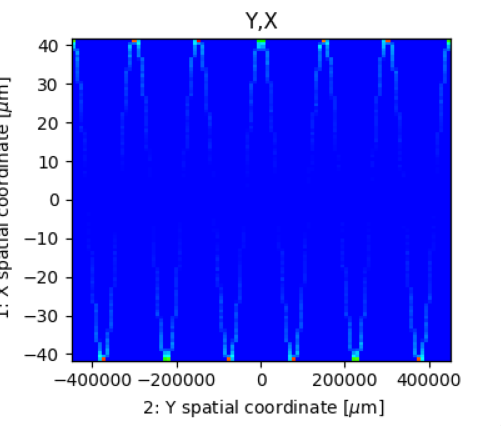
\includegraphics[width=0.49\textwidth]{wigglers/fig4a.png}

\includegraphics[width=0.49\textwidth]
{wigglers/fig4b.png}
\end{figure}

